\documentclass[10pt,a4paper]{report}
\addtolength{\textheight}{-4cm}
\addtolength{\textwidth}{+2cm}
%------------------------------------------------------------------------------------------------------
\usepackage{xltxtra,fontspec,xunicode}
\usepackage[slantfont,boldfont]{xeCJK} % 允许斜体和粗体

\setCJKmainfont{WenQuanYi Micro Hei}             % 缺省中文字体
\setCJKmonofont{WenQuanYi Micro Hei Mono}        % 中文等宽字体
\setmainfont{DejaVu Serif}                       % 英文衬线字体
\setsansfont{DejaVu Sans}                        % 英文无衬线字体
\setmonofont{Monaco}                             % 英文等宽字体
%-------------------------------------------------------------------------------------------------------
\linespread{1.3}                                 % 1.5倍行距,值1.6产生双倍行距
% \setlength{\parindent}{0pt}                    % 段落首行缩进
\setlength{\parskip}{1ex plus 0.5ex minus 0.2ex} % 段落间距为1ex,可让TeX在+0.5到-0.8范围内微调
                                                 % 即实际范围在0.8ex~1.5ex之间
%-------------------------------------------------------------------------------------------------------
% 页眉与页脚设置
\usepackage{fancyhdr}
\pagestyle{fancy}
\fancyhf{}                                       %清空页眉页脚
\fancyhead[LE,RO]{\thepage}                      %页眉偶数页左,奇数页右
\fancyhead[RE]{\leftmark}                        %页眉偶数页右
\fancyhead[LO]{\rightmark}                       %页眉奇数页左
% \fancyfoot[LE,RO]{\thepage}                    %页脚偶数页左,奇数页右
% \fancyfoot[RE]{\leftmark}                      %页脚偶数页右
% \fancyfoot[LO]{\rightmark}                     %页脚奇数页左
\fancypagestyle{plain}{                          %重定义plain页面样式
    \fancyhf{}
    \renewcommand{\headrulewidth}{0pt}
}
%-------------------------------------------------------------------------------------------------------
% listings 与 xcolor 配合实现源代码的语法高亮
\usepackage{xcolor}
\usepackage{listings}
\lstset{
	language=Java,
	frame = shadowbox,
	basicstyle = \ttfamily\small,
	columns = fixed,
	numbers = left,
	numberstyle = \footnotesize,
	stepnumber = 1,
	tabsize = 2,
	showspaces = false,
	showstringspaces = false,
	showtabs = false,
	captionpos = b,
	breaklines = tr[],
	breakatwhitespace = false,
	backgroundcolor = \color{white},
	keywordstyle=\color{blue},
	numberstyle=\color[RGB]{0,192,192},
	commentstyle=\color[RGB]{0,96,96},
	stringstyle=\ttfamily\slshape\color[RGB]{128,0,0},
	escapeinside=``
}
%-------------------------------------------------------------------------------------------------------
\usepackage{graphicx}                            % 引入图片
\graphicspath{{img/}{images/}}                   % 要导入的图片的位置。可以有多个目录,但就算只有一个目录,也要用两级花括号
%-------------------------------------------------------------------------------------------------------
	\title{Agile Java}                             % 文章的标题
	\author{                                     % 作者与致谢
		阿左 \thanks{感谢读者} \and 
		Nobody \thanks{感谢国家}
	}
	\date{\today}                                % 日期
	
%-------------------------------------------------------------------------------------------------------
\begin{document}
	\maketitle                                   % 制作标题
	\tableofcontents                             % 生成章节目录
	\setcounter{tocdepth}{5}                     % 生成章节的目录深度
	\listoffigures                               % 生成图片目录
	\listoftables                                % 生成表格目录



	\part{基础入门}

		
\chapter{开发环境}

\section{开发环境配置}


\section{编写第一个ant程序}




		
\chapter{起步}

\section{project元素}

	一个ant文件中一定要有一个project元素。name属性定义工作名字;default属性代表默认启动target;description属性定义说明文本。

	\lstinputlisting[language=XML]{src/02/build.01.xml}

\section{target元素}

	target元素一定要有name属性。

	\subsection{depends属性}

		表示当前target执行依赖于其他的target成功执行。可以有多个depends之间用“,”分隔。

		\lstinputlisting[language=XML]{src/02/build.01.xml}

	\subsection{if属性}

		验证执行前必须设定的属性。例如设定JDK:

		\lstinputlisting[language=XML]{src/02/build.03.xml}

	\subsection{unless属性}

		没有设置才执行

		\lstinputlisting[language=XML]{src/02/build.04.xml}

\section{property元素}

	property可以看作为参数或是变量的定义。可以在构建文件中通过property元素建立,也可以在构建文件外建立一个build.property文件来存放。

	\lstinputlisting[language=XML]{src/02/build.05.xml}

\section{task元素}
	
	task元素是一系列完成指定功能的脚本和程序。比如自带的编译用的javac、打包用的jar、建立目录的mkdir等。用户也可以编写自己的task。


\section{命令行使用ant}

	\subsection{指定文件}

		\verb|-buildfile|或\verb|-file|或\verb|-f|都可以。

	\subsection{显示任务描述}

		\verb|-projecthelp|。

	\subsection{指定变量的值}

		\verb|-D<property>=<value>|


		\chapter{核心类型}

\section{断言类型:Asseritions Type}

	断言类型指定哪些类需要让ant工具执行java断言。enableSystemAssertions属性设定是否允许系统断言,默认为unspecified。

	断言类型内还可以定义enable类型与disable类型,通过这两个类型的class属性与package属性来设置指定的类或是包是否可以执行断言。
	
	允许所有的用户代码执行断言:

	\lstinputlisting[language=XML,firstline=5,lastline=8]{src/03/build.01.xml}

	只允许Test这个类执行断言:

	\lstinputlisting[language=XML,firstline=9,lastline=11]{src/03/build.01.xml}

	允许一个包下所有的类都执行断言:

	\lstinputlisting[language=XML,firstline=13,lastline=15]{src/03/build.01.xml}

	更复杂的定义:

	\lstinputlisting[language=XML,firstline=17,lastline=21]{src/03/build.01.xml}

	引用一个已经存在的定义:

	\lstinputlisting[language=XML,firstline=23,lastline=27]{src/03/build.01.xml}

\section{匹配模式:PatternSet}

	\subsection{包含与排除}

		匹配格式通过以下四个属性指定包含与排除:

		include属性:可以指定多个模式用逗号或空格分隔,相当于一个列表。

		includesfile属性:指定具体包含的文件。可以引用在properties文件中指定的内容。

		exclude属性:和上面的相反。

		excludesfile属性:和上面的相反。

	\subsection{过滤的模式}

		以上四个属性都有三个属性来匹配指定的内容:

		name属性:文件名、路径或格式。

		if属性:指定的属性有定义则生效。

		unless属性:指定的属性没有定义则生效。


	\subsection{例子}

		类名中不包含Test的类:

		\lstinputlisting[language=XML,firstline=5,lastline=8]{src/03/build.02.xml}

		引用已经定义的模式:

		\lstinputlisting[language=XML,firstline=10,lastline=10]{src/03/build.02.xml}

		可以包含多个定义:

		\lstinputlisting[language=XML,firstline=12,lastline=16]{src/03/build.02.xml}

		指定文件名中包含了"some-file"的文件:

		\lstinputlisting[language=XML,firstline=18,lastline=20]{src/03/build.02.xml}

		也可以简写成下面的格式:

		\lstinputlisting[language=XML,firstline=22,lastline=22]{src/03/build.02.xml}

		配合if条件的形式:

		\lstinputlisting[language=XML,firstline=24,lastline=26]{src/03/build.02.xml}

\section{匹配目录:DirSet}

	DirSet类似于PatternSet,用于匹配目录。必填属性dir用于指定一个目录。
	
	DirSet可以引用已经存在的PatternSet,也可以直接使用include、includesfile、exclude、excludesfile属性。

	另外,DirSet还有casesensitive属性来设置是否大小写敏感;followsymlinks属性来设置采用操作系统差异(如linux与windows的路径符号)等。

	定义目录集合的例子:

	\lstinputlisting[language=XML,firstline=5,lastline=19]{src/03/build.03.xml}

\section{匹配目录:FileSet}

	\subsection{设置匹配}

		FileSet匹配符合的文件,它不仅包含DirSet的属性外,还有一些其他的属性:

		file属性:指定单个文件,fileSet定义中至少要dir属性或是file属性。

		defaultexcludes:当值为yes时默认忽略指定的文件(如版本控制文件),常用的模式有:

		\verb|**/*~, **/#*#, **/.#*, **/%*%, **/._*, |

		\verb|**/CVS, **/CVS/**, **/.cvsignore, |

		\verb|**/SCCS, **/SCCS/**, **/vssver.scc, |

		\verb|**/.svn, **/.svn/**, **/.DS_Store |

	\subsection{过滤筛选:selector}

		selector可以看作是FileSet中的一个元素。有以下几种常见的过滤工具:

	\subsection{内容过滤:contains}

		只选择包含text属性定义字符串的文件。

		text属性:文件包含的字符串,不能为空。

		casesenitive属性:大小写敏感。

		ignorewhitespace属性:忽略空白字符。

		\lstinputlisting[language=XML,firstline=21,lastline=23]{src/03/build.03.xml}

	\subsection{时间过滤:date}

		datetime属性:指定时间格式为:MM/DD/YYYY HH:MM AM 。例如:09/09/2006 10:10 am

		milis属性:指定亳秒时间。datetime与milis两个必选一个。

		when属性:文件修改时间的比较方式,默认为equals。其他值还有:before与after。

		granularity属性:允许的时间误差毫秒数。

		pattern属性:指定datettime是否兼容Java中的SimpleDateFormat格式。

		checkdirs属性:是否检查文件目录创建时间,默认为false。

		\lstinputlisting[language=XML,firstline=25,lastline=27]{src/03/build.03.xml}

	\subsection{比较过滤:depend}
		
		比较两个目录下同名的文件,选择最后修改的那个。

		targetdir属性:指定进行比较的目录。

		granularity属性:允许的时间误差毫秒数。

		比较1.4版与1.5版中有修改过的源文件。

		\lstinputlisting[language=XML,firstline=29,lastline=31]{src/03/build.03.xml}

	\subsection{深度过滤:depth}
		
		min最小与max最大。

		\lstinputlisting[language=XML,firstline=33,lastline=35]{src/03/build.03.xml}

	\subsection{差异过滤:different}

		比较目录下的文件中否有不同(当前目录和一层子目录)。比较的内容有:

		1)一个地方有另一个地方没有。
		
		2)文件大小不同。

		3)ignoreFileTimes不为off,且文件修改时间不同。

		4)ignoreContents为true,内容不同。

		属性有:targetdir、granularity(允许的时间误差范围)、ignoreFileTimes、ignoreContents。

		\lstinputlisting[language=XML,firstline=37,lastline=39]{src/03/build.03.xml}

	\subsection{文件名过滤:filename}

		主要属性:name(文件名匹配)、casesensitive、negate(反选,选中不匹配的)。

		例如,选择所有的css样式文件:

		\lstinputlisting[language=XML,firstline=41,lastline=43]{src/03/build.03.xml}
		
	\subsection{目录过滤:paresent}

		选择一个与当前目录对应的目录(targetdir),找出指定目录中不存在或是两个目录中都存在的文件。主要属性有:

		present属性:值为srconly本目录有面targetDir没有的文件;值为both选中两个目录都有的文件。

		\lstinputlisting[language=XML,firstline=45,lastline=47]{src/03/build.03.xml}

	\subsection{正则过滤:containsregexp}

		\lstinputlisting[language=XML,firstline=49,lastline=51]{src/03/build.03.xml}

	\subsection{大小过滤:size}

		value属性:值。

		units属性:单位。以1000为进制的K,M,G。或是以1024为单位的Ki,Mi,Gi。默认为bytes。

		when属性:more,less,equal。

		\lstinputlisting[language=XML,firstline=53,lastline=58]{src/03/build.03.xml}

	\subsection{类型过滤:type}
		
		指定是文件(file)还是目录(dir)。

		\lstinputlisting[language=XML,firstline=60,lastline=62]{src/03/build.03.xml}

\section{文件列表:FileList}

	\lstinputlisting[language=XML,firstline=64,lastline=72]{src/03/build.03.xml}

\section{文件过滤器:FilterSet}
	
	过滤器可以在对文件进行复制或移动时对文件内容进行替换操作。

	\subsection{主要属性}

		1)begintoken属性:用一个字符(默认为@)指定过滤字符串的开始。如:@DATE@

		2)endtoken属性:定义结束。

		3)recurse属性:是否查找多个替换标记,默认为true。

	\subsection{替换版权与日期的例子}

		\lstinputlisting[language=XML,firstline=5,lastline=19]{src/03/build.04.xml}
		
		可引用的版本:

		\lstinputlisting[language=XML,firstline=21,lastline=39]{src/03/build.04.xml}
		
	\subsection{把替换的内容放在属性文件中}

		要替换的文本:

		\lstinputlisting[language=XML,firstline=1,lastline=2]{src/03/src/src.txt}

		属性文件:

		\lstinputlisting[language=XML,firstline=1,lastline=1]{src/03/abc.properties}

		构建文件:

		\lstinputlisting[language=XML,firstline=41,lastline=52]{src/03/build.04.xml}
		
\section{属性集合:PropertySet}

	定义一套可以组其他标签引用的属性集合。

	\subsection{属性与功能}
		
		dynamic属性:是否动态地加载属性。

		negate属性:取反默认为false,如果为true代表返回除PropertySet外的属性。

	\subsection{引用已经存在的属性}

		Propertyref类型可以引用一个已经定义的property。主要属性有:

		name属性:引用的名字。

		prefix属性:引用指定开头的多个属性。

		regex属性:用正则匹配。

		builtin属性:引用ant内建的属性,值为all时表示所有内建属性。

	\subsection{使用属性集合的例子}

		组建一个属性集合:

		\lstinputlisting[language=XML,firstline=5,lastline=11]{src/03/build.05.xml}
		
		projectset间相互引用的例子:
		
		\lstinputlisting[language=XML,firstline=13,lastline=24]{src/03/build.05.xml}
		
\section{文件映射:mapper}

	用来定义文件之间的对应关系的,主要属性有:

	type属性:定义一个实现的类型,可以用现成的也可以自己实现一个。

	classname属性:通过类名指定一个实现类型。type和classname一定要选一个。

	classpath属性:查找类的路径。

	classpathref属性:引用已经有的path作为classpath。

	from属性:源文件的位置。

	to属性:目标文件的位置。

	对于文件映射,不同的实现类提供了不同的映射实现方法,以下各小节是现有的实现。每个类的调用都可以通过类名调用与type属性调用两种方法来写:

	\subsection{identity}

		源文件与目标文件同名。只取文件名,忽略路径:
		
		\lstinputlisting[language=XML,firstline=5,lastline=12]{src/03/build.06.xml}

	\subsection{flatten}

		忽略目录把文件放到一个压缩文件中:
		
		\lstinputlisting[language=XML,firstline=15,lastline=22]{src/03/build.06.xml}

	\subsection{glob}

		匹配路径与文件名:
		
		\lstinputlisting[language=XML,firstline=25,lastline=32]{src/03/build.06.xml}

	\subsection{merge}

		把源文件打包到压缩文件中:
		
		\lstinputlisting[language=XML,firstline=35,lastline=42]{src/03/build.06.xml}

	\subsection{regexp}

		通过正则来映射:
		
		\lstinputlisting[language=XML,firstline=45,lastline=52]{src/03/build.06.xml}

	\subsection{package}

		替换目录名称。
		
		\lstinputlisting[language=XML,firstline=55,lastline=62]{src/03/build.06.xml}

	\subsection{composite}

		多个mapper都对源文件进行操作。Composite Mapper不能通过Mapper类型的type属性定指定:
		
		\lstinputlisting[language=XML,firstline=65,lastline=72]{src/03/build.06.xml}

	\subsection{chained}

		包含多个mapper,源文件依次经过每个mapper操作。
		
		\lstinputlisting[language=XML,firstline=75,lastline=88]{src/03/build.06.xml}

	\subsection{filtermapper}

		对文件名进行过滤:
		
		\lstinputlisting[language=XML,firstline=91,lastline=96]{src/03/build.06.xml}
	
\section{压缩文件:zip}
	
	有两种压缩文件:

	1)当使用src属性时,目录下的文件会以.zip文件格式进行组织。

	2)当使用dir属性时,目录下的文件会以文件系统形式进行组织。

	\subsection{属性与功能}
		
		prefix属性:文件路径前缀,符合的会被选中。

		fullpath属性:包含全路径。

		src属性:用于替代当前的目录位置。

		filemode属性与dirmode属性:文件的权限,如linux下的权限777。

	\subsection{例子}

		以zip格式压缩htdocs/manual目录下的所有文件。存放到docs/user-guide目录下。

		同时添加ChangeLog27.txt文件到zip文件的docs目录下。

		这个zip文件还包含example.zip文件。example.zip文件包含docs/examples目录及其子目录下的所有html文件。
		
		\lstinputlisting[language=XML,firstline=5,lastline=12]{src/03/build.07.xml}

\section{过滤链与过滤读取器:FilterChains and FilterReader}

	一组有序的FilterReader组成FilterChains,用户可以实现自己的FilterReader。

	FilterReader通过classname属性指定实现类。

	在ant任务concat、copy、loadFile、loadProperties、move中都可以直接使用FilterChain进行过滤操作。
		
	\lstinputlisting[language=XML,firstline=5,lastline=21]{src/03/build.08.xml}

\section{定制与扩展}

	用户可以定制的有:conditions、selecters和filters类型。

	\subsection{定制条件判断:Condition}

		实现一个判断字符串是大写的条件判断:

		\lstinputlisting[language=Java]{src/03/src/exp/ant/AllUpperCaseCondition.java}

		构建文件中通过typedef导入,然后使用定义的类。
		
		\lstinputlisting[language=XML,firstline=5,lastline=11]{src/03/build.09.xml}

	\subsection{定制选择器:Selector}

		\lstinputlisting[language=Java]{src/03/src/exp/ant/JavaSelector.java}
		
		\lstinputlisting[language=XML,firstline=13,lastline=21]{src/03/build.09.xml}

		ant已经提供了一个BaseSelector做了一些预处理功能:setError(String errMsg)可提供出错信息;validate()方法会在isSelected()前进行验证。

	\subsection{定制过滤器:Filter}


		\lstinputlisting[language=Java]{src/03/src/exp/ant/RevomeOddCharacters.java}

		直接通过类名调用:
		
		\lstinputlisting[language=XML,firstline=23,lastline=27]{src/03/build.09.xml}


	\part{工具整合}

	\part{实践}


% \chapter{基本使用}
% 
% 	\section{常用的格式}
% 
% 		\subsection{基本的段落}
% 			空行可以自然分隔段落:
% 
% 			可以设定字体为\textit{斜体};给文字加上\underline{下划线}。可以设定字体为\textit{斜体};给文字加上\underline{下划线}。可以设定字体为\textit{斜体};给文字加上\underline{下划线}。可以设定字体为\textit{斜体};给文字加上\underline{下划线}。
% 
% 			可以设定字体为\textit{斜体};给文字加上\underline{下划线}。可以设定字体为\textit{斜体};给文字加上\underline{下划线}。可以设定字体为\textit{斜体};给文字加上\underline{下划线}。可以设定字体为\textit{斜体};给文字加上\underline{下划线}。
% 
% 			可以设定字体为\textit{斜体};给文字加上\underline{下划线}。可以设定字体为\textit{斜体};给文字加上\underline{下划线}。可以设定字体为\textit{斜体};给文字加上\underline{下划线}。可以设定字体为\textit{斜体};给文字加上\underline{下划线}。
% 
% 		\subsection{边注与脚注}
% 			按照国际惯例,这里是鬼扯的部分。\footnote{我才不承认这是为了骗稿费呢~}
% 
% 			同样也给内容加上连注。但边注是没有编号的,因为就在旁边。\marginpar{这里是边注的内容。}
% 
% 		\subsection{原文照排}
% 			在正文中放入源文照排:在Linux下通过\verb|ls -al|查看当前目录下所有文件。
% 
% 			多行的原文照排要用到verbatim环境:
% 			\begin{verbatim}
% 				/* 输出10行"Hello, world!"的面试题 */
% 				/* 某位童鞋的答案是这样写的        */
% 				printf("Hello, world!");
% 				printf("Hello, world!");
% 				printf("Hello, world!");
% 				printf("Hello, world!");
% 				printf("Hello, world!");
% 				printf("Hello, world!");
% 				printf("Hello, world!");
% 				printf("Hello, world!");
% 				printf("Hello, world!");
% 				printf("Hello, world!");
% 			\end{verbatim}
% 
% 			原文照排时强调空格到verbatim*环境:
% 			\begin{verbatim*}
% 				printf("Hello, world!");
% 			\end{verbatim*}
% 
% 		\subsection{程序代码}
% 
% 			使用listings宏包的效果:
% 
% \begin{lstlisting}[language=C]
% #include <stdio.h>
% 
% int main(int argc, char ** argv)
% {
% 	printf("Hello world!\n");
% 	/** 看起来直接用listings和xelatex配合显示中文没有问题 **/
% 	printf("显示中文!\n");
% 	return 0;
% }
% \end{lstlisting}
% 
% 			可以只引用整个代码中的一部分:
% 
% \begin{lstlisting}[language=C,firstline=3,lastline=9]
% #include <stdio.h>
% 
% int main(int argc, char ** argv)
% {
% 	printf("Hello world!\n");
% 	/** 看起来直接用listings和xelatex配合显示中文没有问题s1l1O0O0 **/
% 	printf("显示中文!\n");
% 	return 0;
% }
% \end{lstlisting}
% 
% 			使用\verb|\lstinputlisting|引用外部文件:
% 
% 			\lstinputlisting[language=HTML,firstline=2,lastline=8]{src/aa.html}
% 
% 	\section{图片与表格}
% 
% 		\subsection{使用图片}
% 
% 			试试使用浮动环境插入图片,但是这样图片就不知道浮动到什么地方去了:
% 
% 			\begin{figure}[htbp]                        % 
% 				\centering                              % 图片居中	
% 				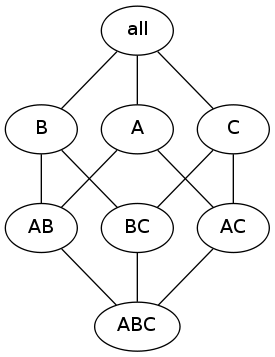
\includegraphics[scale=0.5]{dm0201.png} % scale指定缩放
% 				\caption{第一张浮动的图片}            % 图片的标题,会自动编号
% 				\label{dm0201}                % 图片的标记,一定要加在caption后面。不然指向的是前一个插图
% 			\end{figure}
% 
% 			试试使用浮动环境插入图片,但是这样图片就不知道浮动到什么地方去了:
% 
% 			\begin{figure}[htbp]                        % 
% 				\centering                              % 图片居中	
% 				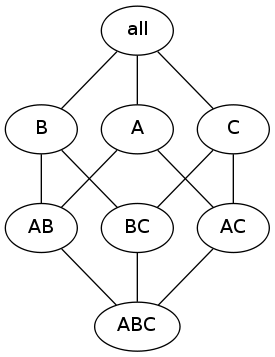
\includegraphics[scale=0.5]{dm0201.png} % scale指定缩放
% 				\caption{第二张浮动的图片}            % 图片的标题,会自动编号
% 				\label{dm0202}                % 图片的标记,一定要加在caption后面。不然指向的是前一个插图
% 			\end{figure}
% 
% 			试试使用浮动环境插入图片,但是这样图片就不知道浮动到什么地方去了:
% 
% 			\begin{figure}[htbp]                        % 
% 				\centering                              % 图片居中	
% 				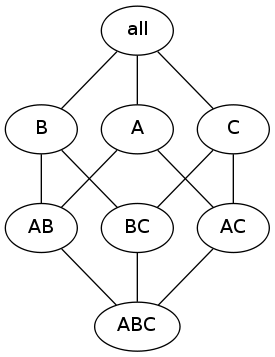
\includegraphics[scale=0.5]{dm0201.png} % scale指定缩放
% 				\caption{第三张浮动的图片}            % 图片的标题,会自动编号
% 				\label{dm0203}                % 图片的标记,一定要加在caption后面。不然指向的是前一个插图
% 			\end{figure}
% 
% 		\subsection{使用表格}
% 
% 			组表格也加上浮动环境:
% 
% 			\begin{table}[htbp]
% 				\caption{浮动环境中的三线表}
% 				\label{tab:threesome}
% 				\centering
% 				\begin{tabular}{lll}
% 					\hline
% 					操作系统 & 发行版 & 编辑器 \\
% 					\hline
% 					Windows & MikTeX & TeXnicCenter \\
% 					Unix/Linux & TeX Live & Emacs \\
% 					Mac OS & MacTeX & TeXShop \\
% 					\hline
% 				\end{tabular}
% 			\end{table}
% 

\end{document}
